%Master File:lectures.tex


\lesson{Gaussian Processes}
\vspace{-1cm}
\begin{center}
  \includegraphics[height=10cm]{GaussianProcessFit-3}
\end{center}
\keywords{Gaussian Processes, regression}
%%%%%%%%%%%%%%%%%%%%%%% Next Slide %%%%%%%%%%%%%%%%%%%%%%%
\renewcommand{\Outline}{%
\begin{slide}
\section[1]{Outline}

\begin{minipage}{10cm}\raggedright
  \begin{enumerate}\squeeze
    \outlineitem{Introduction}{intro}
    \outlineitem{Gaussian Processes}{gp}
    \outlineitem{Bayesian Inference}{bayesgp}
    \outlineitem{Hyper-parameters}{hyperp}
  \end{enumerate}
\end{minipage}\hfill
\begin{minipage}{12cm}
  \includegraphics[width=12cm]{GaussianProcess2D}
\end{minipage}
\end{slide}
\addtocounter{outlineitem}{1}
}

\setcounter{outlineitem}{1}
%%%%%%%%%%%%%%%%%%%%%%% Next Slide %%%%%%%%%%%%%%%%%%%%%%%
\Outline % Introduction
\toptarget{firstoutline}
%%%%%%%%%%%%%%%%%%%%%%% Next Slide %%%%%%%%%%%%%%%%%%%%%%%

\begin{slide}
\section{Gaussian Proccesses}

\begin{PauseHighLight}
  \begin{itemize}
  \item Gaussian processes (GPs) are a mathematically defined ensemble
    of functions\pause
  \item They can be combined with Bayesian inference to give one of the
    most powerful regression techniques\pause
  \item Although Bayesian they can be used in a black-box fashion
    due to the ubiquity of the prior\pause
  \item Mathematically they are a bit complicated\pause{} (because
    Gaussians involve the inverse of matrices which are a real pain to
    work with)\pauseb
  \item In practice they aren't that difficult to use\pause
  \end{itemize}
\end{PauseHighLight}

\end{slide}

%%%%%%%%%%%%%%%%%%%%%%% Next Slide %%%%%%%%%%%%%%%%%%%%%%%

\begin{slide}
\section{Regression}

\begin{PauseHighLight}
  \begin{itemize}
  \item In regression we try to fit a multi-dimensional function to our
    data\pause
  \item (You can use Gaussian Processes for classification, e.g. by
    inferring the probabilities of being in a class, but we ignore this
    as regression is where GP excel)\pause
  \item In regression we have some $p$ dimensional feature vectors
    $\bm{x}_i$ and some target $y_i \in \mathbb{R}$\pause
  \item Our task is to fit a function through all the data points\pause
  \end{itemize}
\end{PauseHighLight}

\end{slide}
%%%%%%%%%%%%%%%%%%%%%%% Next Slide %%%%%%%%%%%%%%%%%%%%%%%

\begin{slide}
\section{Priors on Functions}

\begin{PauseHighLight}
  \begin{itemize}
  \item We can think of a solution as a function $f(\bm{x})$\pause
  \item We can put a prior probability distribution, $p(f)$, on a
    function, $f$, that prefers smooth functions\pause
  \item We can then compute a posterior probability distribution on
    functions given the data, $p(f|\mathcal{D})$\pause
  \item As a likelihood, $p\left(y_i|f(\bm{x}_i)\right)$, we use the
    probability of observing $y_i$ given the true function value is
    $f(\bm{x}_i)$\pause
  \item In general, this would be next to impossible to compute\pause,
    except in the special case where everything is Gaussian (normally)
    distributed\pauseb
  \end{itemize}
\end{PauseHighLight}

\end{slide}

%%%%%%%%%%%%%%%%%%%%%%% Next Slide %%%%%%%%%%%%%%%%%%%%%%%
\Outline % Gaussian Processes
%%%%%%%%%%%%%%%%%%%%%%% Next Slide %%%%%%%%%%%%%%%%%%%%%%%

\begin{slide}
\section{Gaussian Processes}

\begin{PauseHighLight}
  \begin{itemize}
  \item Gaussian Processes are probability distributions over
    functions\pause
  \item (Functions can be viewed as vectors in an infinite dimensional
    vector space)\pause
  \item In the Gaussian Process, $\mathcal{GP}(m, k)$, the probability of
    a function, $f$, is proportional
    \begin{align*}
      p(f|m,k) \propto \E{-\tfrac{1}{2} \int (f(\bm{x})-m(\bm{x})) 
      \, k^{-1}(\bm{x},\bm{y}) \, (f(\bm{y}) -m(\bm{y})) \, \dd \bm{x}
      \, \dd \bm{y}}\pause
    \end{align*}
  \item The function $m(\bm{x})$ is the mean $\av{f(\bm{x})}$ (usually
    taken to be zero in most inference problems)\pause
  \end{itemize}
\end{PauseHighLight}


\end{slide}

%%%%%%%%%%%%%%%%%%%%%%% Next Slide %%%%%%%%%%%%%%%%%%%%%%%

\begin{slide}
\section[-1]{Meaning of GP}

\begin{PauseHighLight}
  \begin{itemize}
  \item To understand GP's we can discretise space, $\bm{x}$, into a
    lattice of points $\{\bm{x}_i\}$\pause
  \item Then (assuming $m(\bm{x})=0$)
    \begin{align*}
      p(f|m,k) \propto \prod_i \E{-\tfrac{f_i^2\, k^{-1}(\bm{x}_i,\bm{x}_i)}{
      2} + f_i  \sum_j
      k^{-1}(\bm{x}_i,\bm{x}_j) f_j}
    \end{align*}
    where $f_i=f(\bm{x}_i)$\pause
  \item We see that the value of the function at each point is normally
    distributed with a mean that depends on functions at neighbouring
    points\pause
  \end{itemize}
\end{PauseHighLight}

\end{slide}


%%%%%%%%%%%%%%%%%%%%%%% Next Slide %%%%%%%%%%%%%%%%%%%%%%%

\begin{slide}
\section[-1]{Covariance function}

\begin{PauseHighLight}
  \begin{itemize}
  \item $k(\bm{x},\bm{y})$ is a covariance function
    \begin{align*}
      \av{\left(\strut f(\bm{x})-m(\bm{x})\right)
      \left(\strut f(\bm{y})-m(\bm{y})\right)} = k(\bm{x},\bm{y})\pause
    \end{align*}
  \item This is sometimes know as a \emph{kernel}\pause---it must be positive
    semi-definite\pause{} (just like in SVMs)\pauseb
  \item It is a free ``parameter'' that the user gets to choose (although we
    can learn its parameters too)\pause
  \item If $k(\bm{x},\bm{y})$ is a function of $\bm{x}-\bm{y}$ it is
    \emph{``stationary''}\pause
  \item If $k(\bm{x},\bm{y})$ is a function of $\|\bm{x}-\bm{y}\|$ it is
    also \emph{``isometric''}\pause
  \end{itemize}
\end{PauseHighLight}

\end{slide}

%%%%%%%%%%%%%%%%%%%%%%% Next Slide %%%%%%%%%%%%%%%%%%%%%%%

\begin{slide}
\section[-2]{Popular Choices of GP Kernel Function}

\begin{PauseHighLight}
  \begin{itemize}
  \item Constant: $\displaystyle k_{\operatorname{C} }(\bm{x},\bm{y})=C$\pause
  \item Gaussian noise: $\displaystyle k_{\operatorname{GN}}(\bm{x},\bm{y})
    =\sigma ^{2}\delta _{\bm{x},\bm{y}}$\pause
  \item Squared exponential: $\displaystyle 
    k_{\operatorname{SE}}(\bm{x},\bm{y})
    =\exp \!\left(-{\frac {\|\bm{x}-\bm{y}\|^{2}}{2\ell^{2}}}\right)$\pause
  \item Ornstein–Uhlenbeck: $\displaystyle 
    k_{\operatorname{OU} }(\bm{x},\bm{y})=\exp \! \left(-{\frac
        {\|\bm{x}-\bm{y}\|}{\ell}}\right)$\pause
  \end{itemize}
\end{PauseHighLight}
\begin{center}
  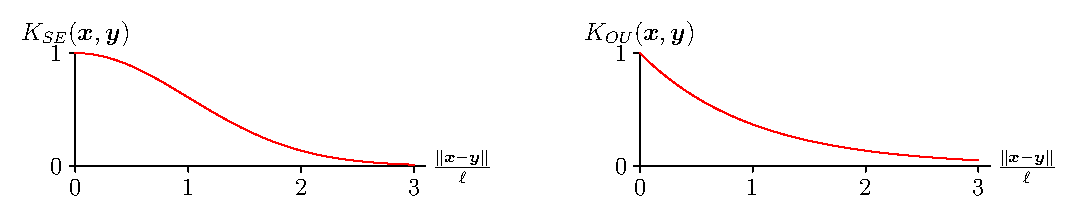
\includegraphics[width=\linewidth]{gp_kernel}
\end{center}

\end{slide}


%%%%%%%%%%%%%%%%%%%%%%% Next Slide %%%%%%%%%%%%%%%%%%%%%%%

\begin{slide}
\section{Gaussian Process Worlds}

\begin{center}
  \includegraphics[width=\linewidth]{GaussianProcess1}\pause
  \\
  \hfill

  \includegraphics[width=\linewidth]{GaussianProcess2}\pauseb
\end{center}
\end{slide}

%%%%%%%%%%%%%%%%%%%%%%% Next Slide %%%%%%%%%%%%%%%%%%%%%%%

\begin{slide}
\section{2-D Gaussian Processes}

\begin{center}
  \includegraphics[width=\linewidth]{GaussianProcess2D}
\end{center}

\end{slide}



%%%%%%%%%%%%%%%%%%%%%%% Next Slide %%%%%%%%%%%%%%%%%%%%%%%
\Outline % Bayesian Inferences
%%%%%%%%%%%%%%%%%%%%%%% Next Slide %%%%%%%%%%%%%%%%%%%%%%%

\begin{slide}
\section[-2]{Observed Gaussian Processes}

\begin{PauseHighLight}
  \begin{itemize}
  \item Given some data points
    $\mathcal{D} = \left( (\bm{x}_i, y_i) \big\vert i=1,\ldots, m
    \right)$ the likelihood (assuming Gaussian error are independence
    of the data point) is given by\vspace*{-0.3cm}
    \begin{align*}
      p(\mathcal{D}| f) = \prod_{i=1}^m
      \mathcal{N}\left(y_i\big\vert f(\bm{x}_i), \sigma^2\right)\pause
    \end{align*}\vspace*{-1.3cm}
  \item Using a Gausssian Process prior we can compute a posterior
    using Bayes's rule\pause
  \item The posterior is a Gaussian Process with a shifted mean and
    variance depending on the data-points\pause
  \item This direct Bayesian derivation gives the answer involving the
    inverse matrix of the correlation function,
    $k^{-1}(\bm{x}, \bm{y})$\pause---this is a pain to work
    with\pauseb
  \end{itemize}
\end{PauseHighLight}

\end{slide}

%%%%%%%%%%%%%%%%%%%%%%% Next Slide %%%%%%%%%%%%%%%%%%%%%%%

\begin{slide}
\section[-2]{Alternative Derivation}

\begin{PauseHighLight}
  \begin{itemize}
  \item Denoting the target values as a vector $\bm{y}$ with elements
    $y_i$\pause
  \item Denoting the matrices of covariances between data points as
    $\mat{K}$ with elements $k(\bm{x}_i,\bm{x}_j)$\pause
  \item Denoting the covariance between the data points and a
    particular position, $\bm{x}_*$ as $\bm{k}_*$ with elements
    $k(\bm{x}_i, \bm{x}_*)$\pause
  \item Denoting the variance a point $\bm{x}_*$ as $k_*=k(\bm{x}_*,
    \bm{x}_*)$\pause
  \item Then the distribution of function values at points at $\bm{x}_i$
    and $\bm{x}_*$ is
    \begin{align*}
      p(\bm{y}, f_*) = \mathcal{N}\!\left(
      \begin{pmatrix}
        \bm{y}  \\ f_*
      \end{pmatrix}
      \bigg \vert \bm{0} ,
      \begin{pmatrix}
        \mat{K} + \sigma^2 \, \mat{I} & \bm{k}_* \\
        \bm{k}_*^\tr & k_*
      \end{pmatrix}\right)\pause
    \end{align*}
  \end{itemize}
\end{PauseHighLight}
\end{slide}

%%%%%%%%%%%%%%%%%%%%%%% Next Slide %%%%%%%%%%%%%%%%%%%%%%%

\begin{slide}
\section{Conditional Probability}

\begin{PauseHighLight}
  \begin{itemize}
  \item To compute the posterior $p(f_*|\bm{y})$ we use
    \begin{align*}
      p(f_*|\bm{y}) = \frac{p(f_*,\bm{y})}{p(\bm{y})}\pause
    \end{align*}
  \item where $p(\bm{y}) = \int p(f_*,\bm{y}) \, \dd f_*$\pause
  \item Because all integrals are Gaussian we can compute the integral
    to obtain
    \begin{align*}
      p(f_*|\bm{y}) = \mathcal{N}\left( f_* \bigg\vert
      \bm{k}_*^\tr(\mat{K} + \sigma^2 \mat{I})^{-1} \bm{y}, 
      k - \bm{k}_*^\tr(\mat{K} + \sigma^2 \mat{I})^{-1} \bm{k}_* \right)\pause
    \end{align*}
  \item Looks complicated, but numerically easy to evaluate\pause
  \end{itemize}
\end{PauseHighLight}


\end{slide}


%%%%%%%%%%%%%%%%%%%%%%% Next Slide %%%%%%%%%%%%%%%%%%%%%%%

\begin{slide}
\section[-2]{$K(x,x') = \exp(-(x-x')^2/(2\,\ell^2))$}
  
\pb\pause\pauselevel{=1}
\begin{center}
  \multipdf[width=\linewidth]{GaussianProcessFit}\pause
\end{center}

\end{slide}

%%%%%%%%%%%%%%%%%%%%%%% Next Slide %%%%%%%%%%%%%%%%%%%%%%%

\begin{slide}
\section{Multi-dimensional Regression}

\begin{PauseHighLight}
  \begin{itemize}
  \item I've shown a 1-D regression example because it is easy to
    visualise\pause
  \item This might be used with a time series\pause
  \item The much more typical situation in machine learning is for
    $\bm{x}$ to have many features so we are doing multi-dimensional
    regression\pause
  \item Gaussian process inference were first used in spatial problems
    where it was known as \emph{krigging}\pause
  \item It was re-invented by the machine learning community who call it
    Gaussian Processes (GP)\pause
  \end{itemize}
\end{PauseHighLight}

\end{slide}


%%%%%%%%%%%%%%%%%%%%%%% Next Slide %%%%%%%%%%%%%%%%%%%%%%%
\Outline % Hyper-parameters
%%%%%%%%%%%%%%%%%%%%%%% Next Slide %%%%%%%%%%%%%%%%%%%%%%%

\begin{slide}
\section[-2]{Choosing the Correct Covariance Function}

\begin{PauseHighLight}
  \begin{itemize}
  \item Choosing the correct covariance function is critical\pause
  \item Most covariance functions include a continuous
    \emph{hyper-parameter} (e.g. the correlation length $\ell$) that we
    have to choose correctly\pause
  \item This is typical of many Bayesian problems were we have some set
    of hyper-parameters, $\bm{\phi}$, describing the model\pause
  \item These are different to the normal parameters we learn
    (e.g. weights $\bm{w}$ or in GP the functions $f(\bm{x}))$\pause
  \item In Bayesian inference we learn the posterior for these normal
    parameters 
    \begin{align*}
      p(f|\mathcal{D},\bm{\phi}) =
      \frac{p(\mathcal{D}| f, \bm{\phi})\, p(f|\bm{\phi})}
      {p(\mathcal{D}|\bm{\phi})}\pause
    \end{align*}
  \end{itemize}
\end{PauseHighLight}

\end{slide}

%%%%%%%%%%%%%%%%%%%%%%% Next Slide %%%%%%%%%%%%%%%%%%%%%%%

\begin{slide}
\section[-2]{Evidence Framework}

\begin{PauseHighLight}
  \begin{itemize}
  \item The normalisation factor, $p(\mathcal{D}|\bm{\phi})$ is known
    as the \emph{marginal likelihood} or \emph{evidence}
    \begin{align*}
      p(\mathcal{D}|\bm{\phi}) =
      \int p(\mathcal{D}| f, \bm{\phi})\, p(f|\bm{\phi}) \, \dd f\pause
    \end{align*}
  \item We can perform a Bayesian calculation at a second level by
    putting a prior on $\bm{\phi}$
    \begin{align*}
      p(\bm{\phi} | \mathcal{D}) = \frac{p(\mathcal{D}|\bm{\phi}) \,
      p(\bm{\phi})}{p(\mathcal{D})}\pause
    \end{align*}
  \item From this we can now marginalise out the hyper-parameters
    \begin{align*}
      p(f|\mathcal{D}) = \int
      p(f|\mathcal{D},\bm{\phi}) \, p(\bm{\phi} | \mathcal{D}) \,
      \dd \bm{\phi}\pause
    \end{align*}
  \end{itemize}
\end{PauseHighLight}

\end{slide}

%%%%%%%%%%%%%%%%%%%%%%% Next Slide %%%%%%%%%%%%%%%%%%%%%%%

\begin{slide}
\section[-2]{Maximum-Likelihood-II}

\begin{PauseHighLight}
  \begin{itemize}
  \item The integral
    \begin{align*}
      p(f|\mathcal{D}) = \int
      p(f|\mathcal{D},\bm{\phi}) \, p(\bm{\phi} | \mathcal{D}) \,
      \dd \bm{\phi}
    \end{align*}
    usually can't be computed analytically and we
    have to use Monte Carlo methods (see later lecture)\pause
  \item An alternative is to use the most likely hyper-parameter\pause
  \item We can find this by using gradient search of
    $p(\mathcal{D}|\bm{\phi})$\pause
  \item This is sometimes referred to as ML-II\pause
  \item Normally even this can be difficult, but for GP its not too
    difficult\pause
  \end{itemize}
\end{PauseHighLight}


\end{slide}

%%%%%%%%%%%%%%%%%%%%%%% Next Slide %%%%%%%%%%%%%%%%%%%%%%%

\begin{slide}
\section{Evidence for GP}

\begin{PauseHighLight}
  \begin{itemize}
  \item For GP the (log)-evidence can be computed in closed form
    \begin{align*}
      \logg{p(\mathcal{D}|\bm{\phi})} = \mypl{1}\pause
      - \frac{1}{2} \bm{y}^\tr (\mat{K}+\sigma^2\mat{I}) \bm{y}
      \pauselevel{=1 :2}\pause
      -   \frac{1}{2}  \logg{|\mat{K}+\sigma^2\mat{I}|}
      \pauselevel{=1 :1, =3 :3}\pause
      - \frac{m}{2} \log(2\,\pi) \pauselevel{=1 :1, =4  :4}\pause
    \end{align*}
    \begin{itemize}
    \item First term measures goodness of fit\mypl{2}
    \item Second term measure complexity of model\mypl{3}
    \item Last term is a common normalisation constant\mypl{4}
    \end{itemize}
  \item Can efficiently compute derivatives and find best parameters\pause
  \item Could overfit!\pauseb
  \end{itemize}
\end{PauseHighLight}


\end{slide}

%%%%%%%%%%%%%%%%%%%%%%% Next Slide %%%%%%%%%%%%%%%%%%%%%%%

\begin{slide}
\section[-2]{Example (slightly pathological)}

\begin{center}
  \includegraphics[width=0.85\linewidth]{marginalLogLikelihoodGP}
\end{center}
\end{slide}

%%%%%%%%%%%%%%%%%%%%%%% Next Slide %%%%%%%%%%%%%%%%%%%%%%%

\begin{slide}
\section{Conclusions}

\begin{PauseHighLight}
  \begin{itemize}
  \item Gaussian processes are very powerful for regression (and
    classification?)\pause
  \item Because all calculations involve Gaussian integrals we can
    compute everything in closed form\pause
  \item (Actually its a pain to do the mathematics because you end up
    working with inverse of matrices)\pause
  \item Fairly generic (black-box) technique because the prior captures
    many continuity constraints\pause
  \item We can use the evidence framework (probability of data) to do model
    selection and hyper-parameter optimisations\pause
  \end{itemize}
\end{PauseHighLight}

\end{slide}

%%% Local Variables:
%%% TeX-master: "lectures"
%%% End:
